\chapter{Introduction}
\label{chap:introduction}

Altough high temperature superconductivity has been known for almost three decades \cite{Bednorz1986}, a satisfactory explanation of this phenomenom still remains as one of the major unsolved problems in theoretical condensed matter physics. 
The discovery of superconductivity in the ceramic copper oxides was a surprising result since ceramic materials, such as the undoped copper oxides, are typically insulators.
However, when doped they can become poor metals and high-temperature superconductors depending on the temperature (See Figure \ref{fig:CuPhaseDiag}). 
The doping is provided either by chemical substitution (e.g. in La$_{2-x}$Sr$_x$CuO$_4$ \cite{Cava1987}) or by changing the oxygen content (as in YBa$_2$Cu$_3$O$_{7-\delta}$ \cite{Wu1987}). 
Doping leads to the appearance of carriers in the Cu-O planes which can be either electrons or holes.
Increasing the carrier concentration leads to conductivity and, for greater carrier concentrations, to superconductivity. 
The value of the superconducting transition temperature (T$_c$) depends strongly on the carrier concentration.
There is characteristic value of carrier concentration that leads to a maximum T$_c$ such that greater dopings produce a decrease in T$_c$.

\begin{figure}[ht]
  \centering
  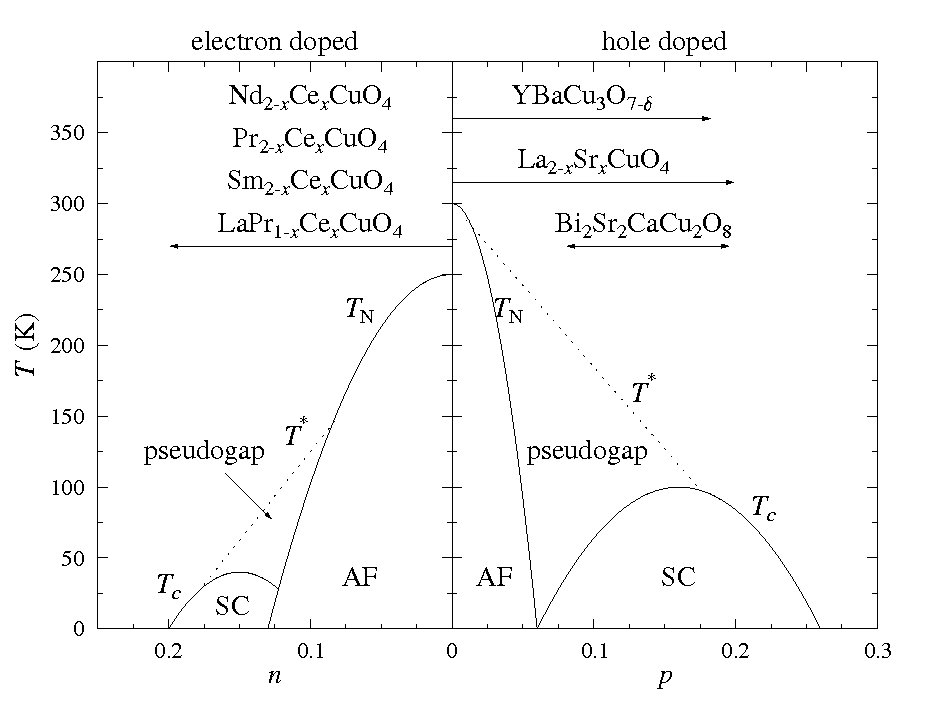
\includegraphics[width=0.8\textwidth]{images/CuPhaseDiag.png}
  \caption[Simplified version of the cuprate superconductor phase diagram]
  {Simplified version of the cuprate superconductor phase diagram \protect\cite{CuPhaseDiag}.}
  \label{fig:CuPhaseDiag}
\end{figure}

Since electrons must be bound together to form Cooper pairs, it was unexpected to find strong electron-electron correlations in copper oxide superconductors. 
One example is given by La$_2$CuO$_4$ which becomes superconducting by replacing some of the trivalent La$^{3+}$ in with the divalent Sr$^{2+}$. 
This insulating material at zero doping becomes a superconductor which is a surprise since band-structure calculations based on the local-density approximation predict the undoped parent compound La$_2$CuO$_4$ to be metallic but it is found to be an antiferromagnetic insulator \cite{Timusk1999}.
This discrepancy is a consecuence of the failure of the independent-particle picture assumed in band calculations and suggests that the undoped parent compounds of the cuprate superconductors are \textit{Mott-Hubbard insulators} \cite{Mott1949}.

Another remarkable feature of the cuprate high-temperature superconductors is the temperature dependence of the normal state resistivity.
In optimally doped materials resistivity shows a linear variation with temperature from T$_c$ to high temperatures (600-1000K) extrapolating to zero resistance at zero degrees \cite{Gurvitch1987}.
In contrast, conventional metals show a resitivity linearly dependent on temperature only for a limited range of temperatures, have an intercept on the temperature axis at some value grater than zero and saturate at high temperatures \cite{Timusk1999}.
The dependency of the resistivity with temperature is different depending on the doping. 
We provide a more detailed review later in this introductory chapter (section \ref{sec:resistivity}) but we emphasize that these resistivity measurements point further to the non-applicability of Fermi-liquid theory\footnote{Fermi-liquid theory describes the excitations in terms of an interacting gas of renormalized quasiparticles.} and of the single-particle picture \cite{Orenstein2000}.

One of the defining properties of a superconductor, within the band energy approximation, is the presence of an energy gap, but early experiments could not find this characteristic signatures in cuprate superconductors.
Instead of abruptly finding a zero density of states below a certain energy at the superconducting transition temperature there was only a partial depression of excitations appearing at a much higher temperature T*.
This region in the phase diagram has been called the \textit{pseudogap phase} and there is evidence for its presence in all cuprate superconductor families \cite{Timusk1999,Muller2007}.
Within the band-theory approximation, a \textit{pseudogap} occurs when some regions of the Fermi surface become gapped while other parts remain conductive. 
With increased doping the gapped portion decreases and the compounds become more metallic. 
The pseudogap seems a fundamental property of underdoped copper oxides however, although it precedes superconductivity for a large part of the phase diagram, its relationship to superconductivity still remains unclear \cite{Basov2005}.

Cuprate superconductors are instrinsically inhomogeneous systems.
For example in La$_{1.85}$Sr$_{0.15}$CuO$_{4}$ and La$_{2}$CuO$_{4.1}$, the dopant atoms, necessary for superconductivity, do not reside at the crystal symmetric sites making these compounds structurally inhomogeneous \cite{Poccia2011}.
In YBa$_2$Cu$_3$O$_{7-\delta}$ (YBCO) the dopant atoms reside in crystal symmetric positions but the departure from stoichiometry produces compositional disorder \cite{Chen1988,Andersen1990} making YBCO also an inhomogeneous system.
Furthermore, even though the dopant atoms are at fixed positions, these structural inhomogeneities have a dynamical character \cite{Mihailovic2005,Bianconi1996}.
Such a dynamical inhomogeneity is present even in some compounds with perfect crystallographic symmetry like HoBa$_{2}$Cu$_{4}$O$_{8}$ \cite{RubioTemprano2000}.

In addition to the breaking of the crystalline translational symmetry the pseudogap phase exhibits other broken symmetries. 
The crystalline rotational symmetry is broken locally in La$_{1.85}$Sr$_{0.15}$CuO$_{4}$ with alternating regions of tetragonal and orthorhombic symmetry \cite{Bianconi1996} according to X-ray absorption spectroscopy. 
Time-reversal symmetry breaking was found using angular resolved photoemission spectroscopy with circularly polarized photons in Bi$_{2}$Sr$_{2}$CaCu$_{2}$O$_{8+\delta}$ \cite{Kaminski2002}. 
The clues provided by these broken symmetries should yield an understanding of the ground state in this pseudogap phase, its elementary excitations and the appearance of superconductivity at temperatures below the onset of the pseudogap. 

One strong motivation for Bednorz and M\"{u}ller to search for superconductivity in Ba$_x$La$_{5-x}$Cu$_5$O$_{5(3-y)}$ was the possibility of strong electron-phonon interactions in oxides due to polaron formation \cite{Bednorz1986}.
Later X-ray absorption experiments found a large oxygen-isotope effect on the pseudogap onset temperature T* which is sign reversed in respect to the isotope effect on T$_c$.
It was also found that there were local deviations on the Cu-O bond lengths appearing at T*.
These is evidence of the significance of electron-lattice interactions in the pseudogap phase and was explained in terms of polaron formation \cite{MustredeLeon1992}.
The formation of polaronic states is a nonadiabatic phenomenon which breaks the Born-Oppenheimer approximation \cite{Born1927}.
Thus, for a complete description of cuprate superconductors, it is impossible to separate the ionic and the electronic motions.

The Bardeen-Cooper-Schrieffer (BCS) theory of superconductivity \cite{Bardeen1957} was developed for and successfully applied to metals within the Fermi-liquid approximation, as such, it seems to lack an appropriate foundation to describe high-temperature superconductivity in copper oxides \cite{Damascelli2003}.
The strong electron-electron correlations prevent successful band structure calculations with independent quasiparticles.
Furthermore the presence of polaronic objects and the observation of lattice and electronic inhomogeneities point to the inadequacy of the Born-Oppenheimer approximation and the reciprocal space formalism.
Such approximations may still remain useful in understanding some aspects of cuprate oxide superconductors but it is clear that there are important features that they are unable to explain.

One approach to explore the electron-lattice dynamics in an inhomogeneous system away from the Born-Oppenheimer (adiabatic) approximation is through model hamiltonians involving both charge and atomic degrees of freedom in real space.
Unfortunately the computationally resources required to deal with such hamiltonians rapidly increase with each degree of freedom introduced thus making unfeasible to explore large systems with many variables.
As such, we are forced to focus on small subsystems in the copper oxide superconductors.
Since there is strong evidence for polaronic behaviour in the O(4)-Cu(1)-O(4) cluster \cite{MustredeLeon1992,Salkola1994} in the YBCO superconductor it seems essential to correctly describe this subsystem using a non-adiabatic hamiltonian in real space.
Furthermore, some models have considered the interaction between fermionic \textit{pairs} and bipolaronic bosonic objects \cite{Bussmann-Holder2005,Mihailovic2001,Bar-Yam1991,doi:10.1142/S0217979200003812} explaining several properties of the normal state in the pseudogap region. 
The bipolaronic objects could arise from the O(4)-Cu(1)-O(4) cluster and couple to fermionic carriers on the CuO$_2$ planes thus raising the importance of correctly describing this subsystem.
A particular model hamiltonian has been used to successfully describe the local inhomogeneities and optical signatures in this cluster as a consecuence of polaron formation \cite{MustredeLeon1992, Salkola1994, Salkola1995,DeLeon1999, Leon2008, MirandaMena2007,Mena2006,MustredeLeon2000}.
Although there is a considerable amount of work on this model hamiltonian, the effect of the polaron formation on the \textit{electronic}\footnote{The departure from the Born-Oppenheimer approximation means that the excitations in the model can not be identifyed as having either a lattice or electronic origin but are always in a \textit{mixed} state of both. Thus, when we refer to an \textit{electronic} excitation we mean an excitation that in the absence of electron-lattice coupling would correspond to the electronic degrees of freedom in the model.} excitations of the model has not been throughly explored.
In this thesis we describe in detail this model hamiltonian and many of its lowest excitations incluiding the electronic excitations.

The remainder of this introductory chapter is devoted to reviewing some of the experimental results pointing to the importance of considering the lattice and electronic inhomogeneities in the description of superconductivity. 
We start, in section \ref{sec:dynamicDistortions} with an overview of the dynamic local lattice distortions in cuprates. 
Afterwards, in section \ref{sec:electronicInhomogeneity}, we turn our attention to electronic inhomogeneities. 
In sections \ref{sec:phonon_spectra} and \ref{sec:specific_heat} we present some experimental anomalies in the phonon spectra and specific heat respectively.
Finally we duscuss some of the experimental results in isotopic effects and ultrafast spectroscopy in sections \ref{sec:isotopic_effects} and \ref{sec:ultrafast_spect} respectively.


\section{Dynamic local lattice distortions}
\label{sec:dynamicDistortions}

All cuprate high-T$_c$ superconductors consist of a given number $n$ of CuO$_2$ planes separated by \textit{charge reservoirs}.
Some materials, such as La$_{2-x}$Sr$_x$CuO$_4$ and Nd$_{2-x}$Sr$_x$CuO$_4$, have one CuO$_2$ plane per unit cell. 
Other compounds like Bi$_2$Sr$_2$Ca$_{n-1}$Cu$_n$O$_{2n+4+x}$ have been synthesized with $n=1,2$ and 3 CuO$_2$ planes \cite{Basov2005}.
In this thesis we give particular attention to YBa$_2$Cu$_3$O$_{7-\delta}$ (YBCO) which has two CuO$_2$ layers and is one of the most commonly studied compounds.

The crystal structure of YBa$_2$Cu$_3$O$_6$ ($\delta=1$) is tretragonal (\textit{P4/mmm} space group) whereas YBa$_2$Cu$_3$O$_7$ ($\delta=0$) is orthorrombic (\textit{Pmmm} space group).
The oxygen atoms in YBCO occupy four inequivalent positions and are usually labelled as follows: O(1) is in the Cu-O \textit{chains}, O(2),O(3) are in the CuO$_2$ \textit{planes}, and O(4) is the \textit{apical} oxygen (see Figure \ref{fig:YBCO_structure}).
Each oxygen contributes in a different way to the several properties of the material.
The sites O(2), O(3), and O(4) are always filled whereas, depending on the value of $\delta$, the population of the O(1) sites varies.
The $\delta$ value depends on the growing and treatment conditions specially on the thermal annealing at different atmospheres or vacuum \cite{Ivanov1995}.
The two copper atoms in the unit cell also occupy two inequivalent positions.
The labels Cu(1) and Cu(2) are usually assigned to copper atoms in the chains and CuO$_2$ planes respectively.
It is commonly accepted that the Cu(1)-O(1) chains serve as reservoirs for excess holes \cite{Pickett1989}. 
At low $\delta$ the holes are localized at the chains and do not contribute to the conductivity at low temperatures however, at larger $\delta$, a hole transfer occurs to the Cu(2)-O(2),O(3) planes and the samples become superconducting \cite{Cava1988}.

\begin{figure}[ht]
  \centering
  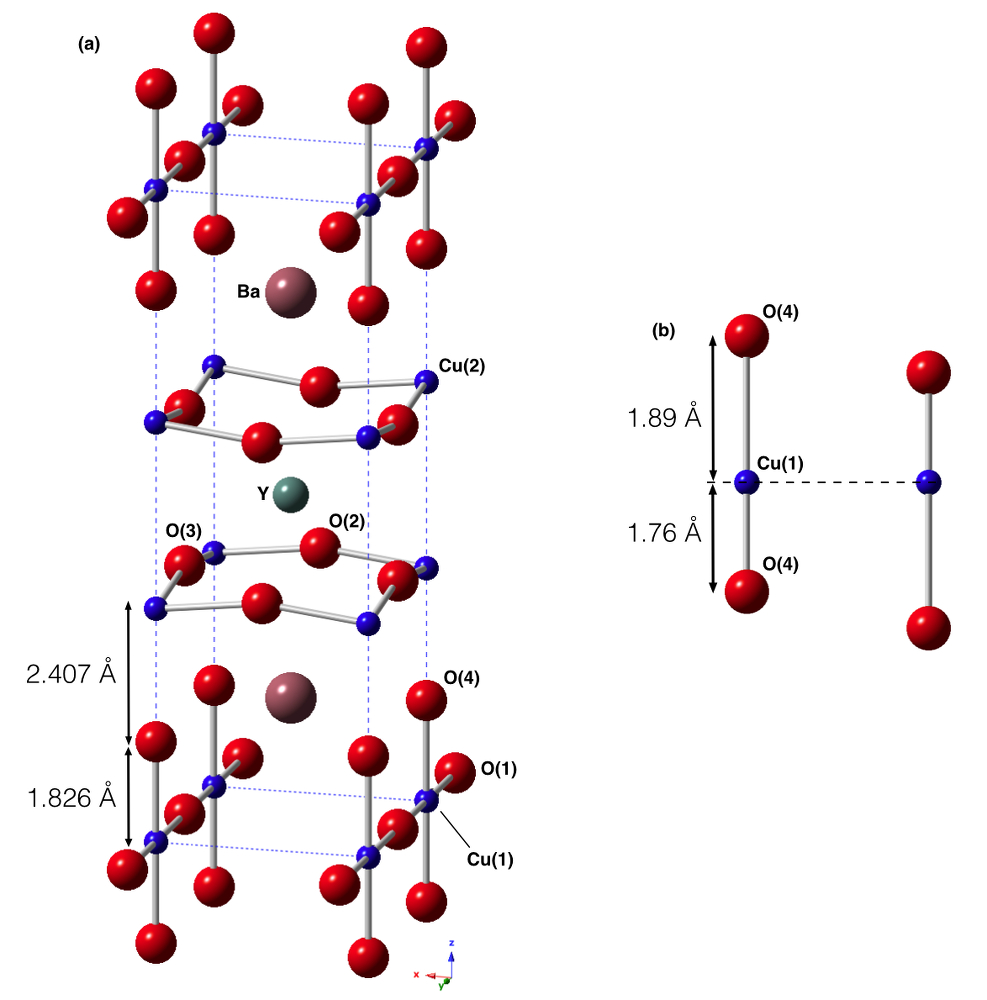
\includegraphics[width=0.7\textwidth]{images/YBCO_O-Cu-O.jpg}
  \caption[Crystal structure of YBa$_{2}$Cu$_{3}$O$_{7}$ and the two possible O(4)-Cu(1)-O(4) configurations.]
  {\textbf{(a)} Crystal structure of YBa$_{2}$Cu$_{3}$O$_{7}$. The dashed line denotes de unit cell. \textbf{(b)} The two possible configurations in the O(4)-Cu(1)-O(4) cluster due to the split O-Cu bond distances (not to scale).}
\label{fig:YBCO_structure}
\end{figure}

Crystal structure in cuprates was determined first by diffraction methods without any sign of significant distortions associated with the in-plane nor with the apical oxygen atoms \cite{Capponi1987,Schafer1988}. 
One of the first observations of a local lattice distortion in cuprates was made using Cu K-edge extended X-ray absorption fine structure (EXAFS) measurements.
It showed a two distances for the Cu(1)-O(4) bond length in YBa$_2$Cu$_3$O$_7$ at temperatures above the superconducting transition temperature, T$_{c}$, with a difference in length close to 0.13 \AA\ \cite{MustredeLeon1990,Conradson1990}.
Since the average bond lengths in diffraction have a significantly higher precision ($\sim 0.001$ \AA\ \cite{Miceli1988}) than local probes like EXAFS \cite{Rehr2000}, these reports were controversial \cite{Kwei1990}.
To resolve the controversy, it was noticed that the time scale in EXAFS measurements is such that dynamical distortions can be measured but, depending on the size of the distortion, elastic techniques like X-ray or neutron diffraction are unable to detect them \cite{Salkola1995}.
For example, it was shown that the two-site O(4) distribution in in Tl$_{2}$Ba$_{2}$CaCu$_{2}$O$_{8}$ could be only detected in a pair distribution function obtained from neutron inelastic scattering but not with that obtained from neutron diffraction \cite{Egami1991}. 
Consequently, it is important to take into account both the spatial resolution and time resolution of the techniques used to study the actual atomic structure of these materials \cite{Mihailovic2005}. 
The explanation of the discrepancies between these results with diffraction and optical spectroscopical results lead to the interpretation of this two-sites Cu(1)-O(4) distribution as a dynamical distortion of polaronic origin \cite{MustredeLeon1992}.

In YBa$_2$Cu$_3$O$_7$ the EXAFS analysis using polarized X-rays on magnetically oriented powders showed two different Cu(1)-O(4) distances diferring by $\sim 0.10-0.13$ \AA\ that changed into a single site distribution in the vicinity of the superconducting transition temperature \cite{Conradson1990,MustredeLeon1992a}. 
This result was also received with skepticism based on earlier diffraction \cite{battlog1992lattice,Kwei1990,Sharma1991} and optical spectroscopy \cite{Thomsen1993} results. 
However, independent EXAFS measurements in other oriented samples \cite{Stern1993} and single crystals \cite{Booth1996} also showed a two-site distribution in YBa$_{2}$Cu$_{3}$O$_{6.7}$, YBa$_{2}$Cu$_{3}$O$_{6.5}$ and Co doped  YBa$_2$Cu$_{2.8}$Co$_{0.2}$O$_{7+\delta}$ \cite{MustredeLeon1991}. 

Similar two site distributions obtained from EXAFS spectra were found for the Cu(2)-O(4) distribution in Bi$_{2}$Sr$_{2}$CaCu$_{2}$O$_{8}$ \cite{bianconni1992lattice} and in TlBa$_{2}$Ca$_{3}$Cu$_{4}$O$_{11}$ \cite{Allen1991} starting at temperatures above T$_{c}$. 
In these compounds (and other cuprates) the average Cu(2)-O(4) bond length lies between 2.49 and 2.73 \AA, which is much longer than the Cu(1)-O(4) bond length in YBa$_{2}$Cu$_{3}$O$_{7}$ ($\sim 1.87$ \AA). 
This fact makes more difficult the identification of details about the O(4) distribution due to the stronger mixing of the Cu(2)-O(4) EXAFS signal with those of other atoms and the increased zero point motion of the O(4) atom due to weaker Cu(2)-O(4) bond compared with the Cu(1)-O(4) bond.
For this reason in most EXAFS studies addressing the O(4) motion a gaussian single site broadened distribution has been used, reporting only changes in the width of the distribution as a function of temperature \cite{Booth1995,Oyanagi2007,Zhang2009}.

In plane Cu(2)-O local lattice distortions were identified in La$_{1.85}$Sr$_{0.15}$CuO$_{4}$ appearing below 100 K \cite{Bianconi1996,Oyanagi2007}, in TIBa$_{2}$CuO$_{6}$ below 120 K \cite{Conradson1997} and in La$_{2}$CuO$_{4.1}$ below 150 K \cite{Lanzara1997,MustredeLeon:xj5003}. 
In this case the observation of such distortions in YBa$_{2}$Cu$_{3}$O$_{7}$ and related compounds becomes more difficult due the similarity in Cu-O bond lengths in the CuO$_2$ planes and chains, whose contributions are mixed in the EXAFS signal \cite{Conradson1997,MustredeLeon1992a}.

As of now only in La$_{1.85}$Sr$_{0.15}$CuO$_{4}$ has been possible to identify local lattice distortions involving both in plane oxygen and apical oxygen atoms  \cite{Bianconi1996}. 
We also stress that from all these EXAFS experiments it is only possible to probe with enough detail the nearest neighbor environment around the Cu atoms, thus the spatial extension of the distortions cannot be determined solely from these measurements. 
Additional structural information \cite{Bianconi1996a} is needed to formulate models about the extension of the distortions as discussed in Ref. \cite{Bianconi1996}.
Pair distribution function analysis of diffraction, X-ray and neutron inelastic scattering can additionally provide information about the intermediate range (up to 10-15 \AA) atomic structure, complementary to the information obtained from EXAFS \cite{Egami2003}. 
Pair distribution function results in La$_{1-x}$Sr$_{x}$CuO$_{4}$ \cite{Bozin1999,Bozin2000} indicate that the atomic structure in this material is a combination of nanoscale regions with different local Cu-O environments, in agreement with the model proposed in Ref. \cite{Bianconi1996}. 
A homogeneous structure only appears when dopant concentrations are above $x = 0.25$. 
In this region the electronic behavior can be described in terms of free fermion quasiparticles.

%Stripes review: \cite{Kivelson2003}
%Very nice review about electrodynamics in High-Tc superconductors: \cite{Basov2005} 

\section{Electronic inhomogeneity}
\label{sec:electronicInhomogeneity}

Although an inhomogeneous electronic ground state does not necessarily follow from structural inhomogeneities, such as the ones discussed in the previous section, for some regions of the phase diagram such state is realized.
Early EXAFS analysis in La$_{1.85}$Sr$_{0.15}$CuO$_4$ and X-ray diffraction in Bi$_2$Sr$_2$CaCu$_2$O$_{8+y}$ showed two orders of the CuO$_6$ octahedra below 100K assigned to two types of \textit{stripes} with different order, one of them with a large tilting and elongation of the in-plane Cu-O distances.
This significant distortion was taken as an indicative that the electronic structure in both kind of stripes is different \cite{Bianconi1996,Bianconi1996a}.
Since then it has been possible to detect the existence of srtipe-ordered phases in La$_2$CuO$_{4+\delta}$, La$_{1.6-x}$Nd$_{0.4}$Sr$_x$CuO$_4$ for $0.05<x\leq 0.2$, La$_{2-x}$Ba$_x$CuO$_4$, La$_{2-x}$Sr$_x$CuO$_4$ for $0.02<x<0.13$, La$_2$CuO$_{4+\delta}$ \cite{Kivelson2003}, Bi$_2$Sr$_2$CaCu$_2$O$_{8+\delta}$ \cite{Poccia2011a} and YBa$_2$Cu$_3$O$_{7-\delta}$ \cite{Mook2002,Haase2003}.
Spatial variations in the densitiy of states have also been measured using scanning tunneling miscroscopy (STM) in Bi$_2$Sr$_2$CaCu$_2$O$_{8+\delta}$ \cite{Pan2001}. 


ARPES review: \cite{Damascelli2003}
\begin{quote}
  angle-resolved photoemission spectroscopy (ARPES) plays a major role because it is the most direct method of studying the electronic structure of solids (see Sec. II). Its large impact on the development of many-body theories stems from the fact that this technique provides information on the single-particle Green’s function, which can be calculated starting from a microscopic Hamiltonian.
\end{quote}

This reference also reviews experimental issues and considerations about detecting stripes

\section{Phonon spectra}
\label{sec:phonon_spectra}

Forbidden ir modes only present below T* \cite{?}

Anomalous ir conductivity in the pseudogap phase \cite{Basov1996}

``Phonon contributions to the specific heat as a function of Co content correlate closely with observed anomalies in calorimetric measurements, indicating that phonons contribute intrinsically to the transition mechanism, e.g. via Bose condensation of structural bipolarons.'' \cite{Obhi1990} 

Raman spectra says: pseudogap is s-wave; superconducting gap is d-wave \cite{Sakai2013}.
Pseudogap is not incipient superconductivity but another kind of order \cite{He2011}

\section{Specific heat}
\label{sec:specific_heat}

Specific heat: \cite{Loram1993}

For a Fermi liquid the specific heat rises linearly with the temperature.

\section{Electric resistivity}
\label{sec:resistivity}

T vs T$^2$ \cite{Timusk1999}!!

For a Fermi liquid the dc resistance varies as T$^2$.

\cite{Muller2007}: \textit{At optimum doping, i.e T$_c$ maximum, and in the normal state, the resistivity increases linearly with temperature}

\cite{Damascelli2003}
\begin{quote}
Even though the approximate T$^2$ dependence of the resistivity observed in the overdoped metallic regime was taken as evidence for Fermi-liquid behavior, the applicability of Fermi-liquid theory (which describes electronic excitations in terms of an interacting gas of renormalized quasiparticles) to the ``normal'' metallic state of high-temperature superconductors is questionable, because many properties do not follow canonical Fermi-liquid behavior (Orenstein and Millis, 2000).
On top of this complexity, it has long been recognized that also the interplay between electronic and lattice degrees of freedom as well as the tendencies towards phase separation are strong in these componds (Sigmund and Muller, 1993; Muller, 2000). 
\end{quote}

\section{Isotopic effects}
\label{sec:isotopic_effects}

It is possible to make a site-selective substitution $^{16}$O $\rightarrow$ $^{18}$O in YBCO \cite{Conder1993} allowing a precise study of the isotopic effects. 
This has effects in both the phonon frequencies \cite{Ruani1994} and T$_{c}$ \cite{Zech1994,Cardona1988}. 
The \textit{harmonic} approximation accounts well for the O(2)/O(3) vibrations but it fails for O(4) (see again \cite{Ruani1994})

Noticeable isotopic shifts have been used to identify particular excitations as \textit{phononic} in origin (v.g. \cite{Thomsen1990}) however, we will argue, the converse is not true. 
That is, there can be \textit{phononic} excitations without a measurable isotopic shift.

From the isotope effects in the London penetration length follows that the carriers are polaronic objects \cite{Zhao1997}.

From \cite{Khasanov2004} \begin{quote}A substantial isotope shift $\Delta\lambda_{ab}/\lambda_{ab}=2.8(1.0)$\% at 4 K is observed, implying that the in-plane effective supercarrier mass $m^*_{ab}$ is oxygen-isotope dependent with $\Delta m^*_{ab} / m^*_{ab}=5.5(2.0)$\%.\end{quote}

Isotope dependence of the electronic energy bands \cite{Gweon2004}

(small) isotope effects on T$_c$ mainly come from in-plane oxygens \cite{Zech1994}

There's no isotope effect on Tc for 16O$\rightarrow$18O in YBCO \cite{Thomsen1988}

\section{Ultrafast spectroscopy}
\label{sec:ultrafast_spect}

\cite{Smallwood2012}: Using femtosecond lasers they study Cooper-pair recombinations in Bi$_2$Sr$_2$CaCu$_2$O$_{8+\delta}$
\begin{quote}Gap and quasiparticle population dynamics revealed marked dependencies on both excitation density and crystal momentum. Close to the d-wave nodes, the superconducting gap was sensitive to the pump intensity, and Cooper pairs recombined slowly. Far from the nodes, pumping affected the gap only weakly, and recombination processes were faster. These results demonstrate a new window into the dynamical processes that govern quasiparticle recombination and gap formation in cuprates.\end{quote}

\section{Scope and outline of this thesis}
\label{sec:scope}

% Lattice inhomogeneities limit the applicability of $k$-space formalism.
% Correlated electron-lattice motion prevents the use of Born-Openheimer approximation

% A Peierls-Hubbard model has been used there to explain the lattice distortion in terms of bipolarons.
% We explore many other excitations in that model trying to reconcile its predictions with the experimental observations.
% Particular emphasis is given to the isotopic effects because there is controversy around them and they probe the electron-lattice relationship.
% We suggest a possible two-component superconductivity model involving bosonic bi-polaronic objects and free fermions. 
% Chapter outline.

Quantum solid-state theory usually assumes a periodic potential however, since these materials are intrinsically inhomogeneous, it is possible that a successful model needs to abandon such assumption. 
This calls into question the applicability of models based on the \textit{reciprocal space} formalism.
Furthermore, some of the experimental results reviewed in the previous secions suggest that the polaronic behaviour must be taken into account.
This correlated electron-lattice movement prevents the use of the Born-Oppenheimer approximation, which splits the system's wavefunction in electronic and lattice factors $\Psi = \psi_{electronic}\psi_{lattice}$.
Some systems with an important electron-lattice interaction can be treated with perturbation theory either assuming a small (adiabatic) or strong (anti-adiabatic) interaction \cite{?}. 
However, it seems that the electron-lattice interaction in the CuO planes for cuprate superconductors falls in the middle of such extremes \cite{MustredeLeon1992} preventing the use of any such approximation.

We are prompted, therefore, to use an exact model free from the approximations described above. 
The computational complexity of exact models forces us to restrict the system under study to a small subset of the whole compound.
In this work we return to a model describing the peculiar polaronic behaviour of the O(4)-Cu(1)-O(4) cluster in YBa$_{2}$Cu$_{3}$O$_{7}$ approximating the cluster as a system with three sites and two holes \cite{MustredeLeon1992}.
Such approximation is justified as the Cu(1)-O(4) bond length (1.83 \AA) is far shorter than the Cu(2)-O(4) bond length ($\sim$ 2.41 \AA) (see Fig. \ref{fig:YBCO_structure}), making charge transfer outside the cluster a much slower process than the charge dynamics inside the cluster. 
This model provides a very simple framework to explore the charge dynamics influenced by the lattice vibrations and has successfully described the split O(4)-Cu(1)-O(4) distance observed by EXAFS experiments (see section \ref{sec:dynamicDistortions} above).
Although we cannot directly identify the three site cluster proposed in this model with a particular structure of the CuO plane, the general approach of charge transfer between hole rich regions and hole poor regions in the plane coupled to the lattice degrees of freedom is still valid, hence the general conclusions we draw from this model applicable to describe the structure of the CuO plane.

It has been found that superconductivity occurs in the Cu(2)-O(2,3) planes rather than the Cu(1)-O(1,4) chains partially addressed by the model under study in this work.
This raises a question about the relevance of the polaronic behaviour, es explored with this model, to superconductivity.
It is indeed beyond the capability of such a simple model to address the nature of high-temperature superconductiity.
However, it is possible that the polaronic objects in the Cu(1)-O(1,4) chains are capable of providing a pairing mechanism for the Cooper pairs in the Cu(2)-O(2,3) planes.
This will point to a \textit{two component superconductivity} theory similar to some current proposals \cite{?}

% Thesis outline here